\section*{Teoretická část}
Budeme sledovat hysterézní smyčky feritů.
Rozeznáváme tři základní typy hysterézních smyček --- úsečku, Rayleighův tvar a normální.

Používáme zapojení na obrázku \ref{o:schema}.

\begin{figure}[htbp]
\centering
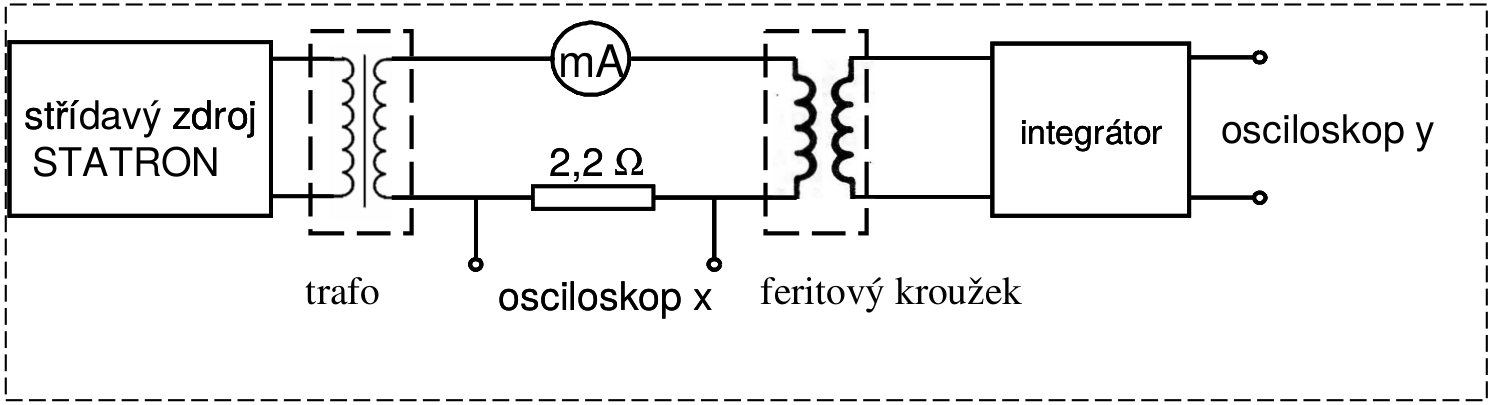
\includegraphics[width=\textwidth-2cm]{graficos/schema}
\caption{Zapojení pro pozorování hysterezních smyček}
\label{o:schema}
\end{figure}

Na miliampérmetru měříme efektivní hodnotu proudu $I_{ef}$, z něj určíme maximální intenzitu magnetického pole v kroužku
\begin{equation}
H_m=\frac{2 n_1 \sqrt{2} I_{ef}}{\pi (d_1+d_2)} \,,
\end{equation}
kde $n_1$ je počet závitů na primárním vinutí a $d_1$ a $d_2$ jsou vnitřní a vnější průměr kroužku.

Koercivní sílu $H_C$ určíme srovnáním s $H_m$ na stínítku osciloskopu.

Abychom mohli určit maximální magnetickou indukci $B_m$, okalibrujeme vertikální osu osciloskopu pomocí střídavého napětí známé velikosti.
Obvod zapojíme podle obrázku \ref{o:kalib} a pustíme do něj střídavé napětí o známé úhlové frekvenci $\omega$.

\begin{figure}[htbp]
\centering
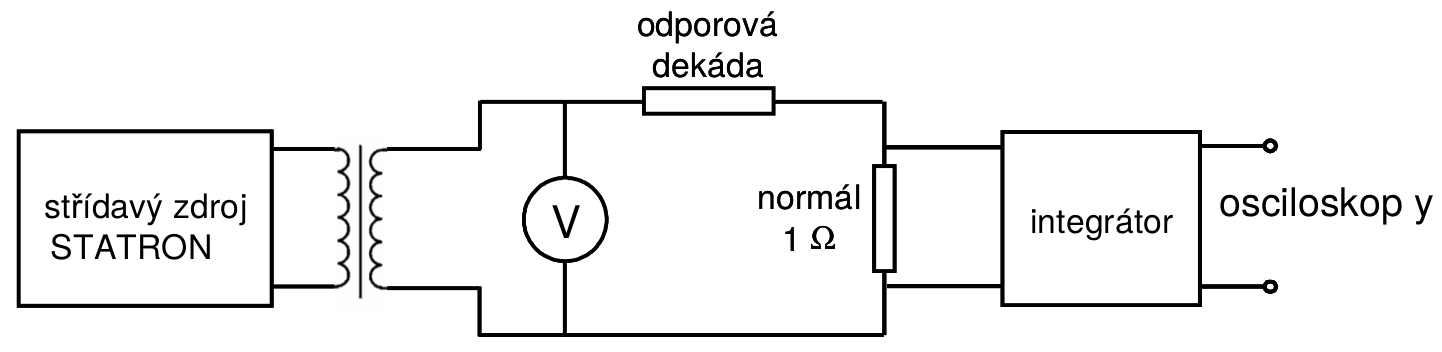
\includegraphics[width=\textwidth-2cm]{graficos/kalib}
\caption{Zapojení pro kalibraci vertikální osy}
\label{o:kalib}
\end{figure}

Na dekádě zvolíme odpor \SI{999}{\ohm}, takže efektivní hodnota napětí na normálu $U_{ef}$ bude rovna jedné tisícině udáje na voltmetru.
$B_m$ určíme jako \cite{skripta}
\begin{equation} \label{e:kalibrace}
B_m=\frac{U_{ef} \sqrt{2}}{\omega S n_2} \,,
\end{equation}
kde $n_2$ je počet závitů na sekundárním vinutí a $S$ je průřez kroužku
\begin{equation}
S=\frac{1}{2} (d_1-d_2) v \,,
\end{equation}
kde $v$ je výška kroužku.
Takto určíme jednu skutečnou hodnotu $B_m$ při plně rozvinuté hysterezní smyčce, ostatní určíme poměrně k ní.